\clearpage
\section{August 2026 Progress Exhibit Gallery}
\label{app:gallery}

These exhibits retain their August 2026 scope. The September public-release
sheet and its audit are shown in Section~\ref{sec:public-release}.
References to current runs within this gallery refer to the August snapshot.

This gallery separates three meanings of scale that should not be collapsed into
one claim. The $10\times10\times10$ hybrid ribbon is the largest coherent
readable strip currently available; the $21\times21\times21$ sheet-book view is
the largest reading-frame exhibit; and the new maintained
$21\times21\times21$ geometry run is the largest canonical pre-fit pile. That
last run stops deliberately after quadribbon concatenation and is not called a
global fit.

\paragraph{Exhibits.} Fit state is kept separate from geometric scale so
a large pre-fit pile cannot be mistaken for a solved global ribbon.
{\small
\begin{itemize}
  \setlength{\itemsep}{0.25em}
  \item \textbf{PHerc0139, $4\times5\times5$:} 100 cubes in the current
  integrated fitted and baked run; visual quality-mask faults fall from 41,407
  to 34,938 (16\%), with zero primary-sheet hard conflicts.
  \item \textbf{PHerc0139, $10\times10\times10$:} 16.444M vertices and
  32.608M faces in the hybrid champion lineage; this is the largest coherent
  readable exhibit, not proof of the current general pre-weld fitter.
  \item \textbf{PHerc0139, $21\times21\times21$:} 9,110 unique world-frame
  meshes, 195.971M vertices, and 381.764M faces; the maintained 6.46-GiB
  stage-1 concat is complete with zero final failures, but fit was not run.
  \item \textbf{PHerc1203, $5\times5\times5$:} 3.984M vertices and 7.753M
  faces; 125/125 cubes complete with zero reject/fail, and 125/125 canonical
  meshes are 2-manifold with zero same-direction defects.
  \item \textbf{PHerc1447, $5\times5\times5$:} 2.170M vertices and 4.191M
  faces under the same guards; 125/125 cubes complete with zero reject/fail,
  and all 125 canonical meshes pass the same topology checks.
\end{itemize}
}


\paragraph{Reproducibility boundary.} The current $21^3$ concat log records an
explicit stop after stage~1; its 9,110-row inventory balances exactly, and 12/12
overlapping cube meshes are byte-identical across the baseline and current
runs. The grid, quadribbon, and manifold self-tests pass, and both prize piles
were meshed with the winding guards armed. The multi-gigabyte VMesh is
represented here by its checksum rather than copied into the paper repository.

\clearpage
\begin{figure*}[p]
  \centering
  \begin{subfigure}[t]{0.94\textwidth}
    \centering
    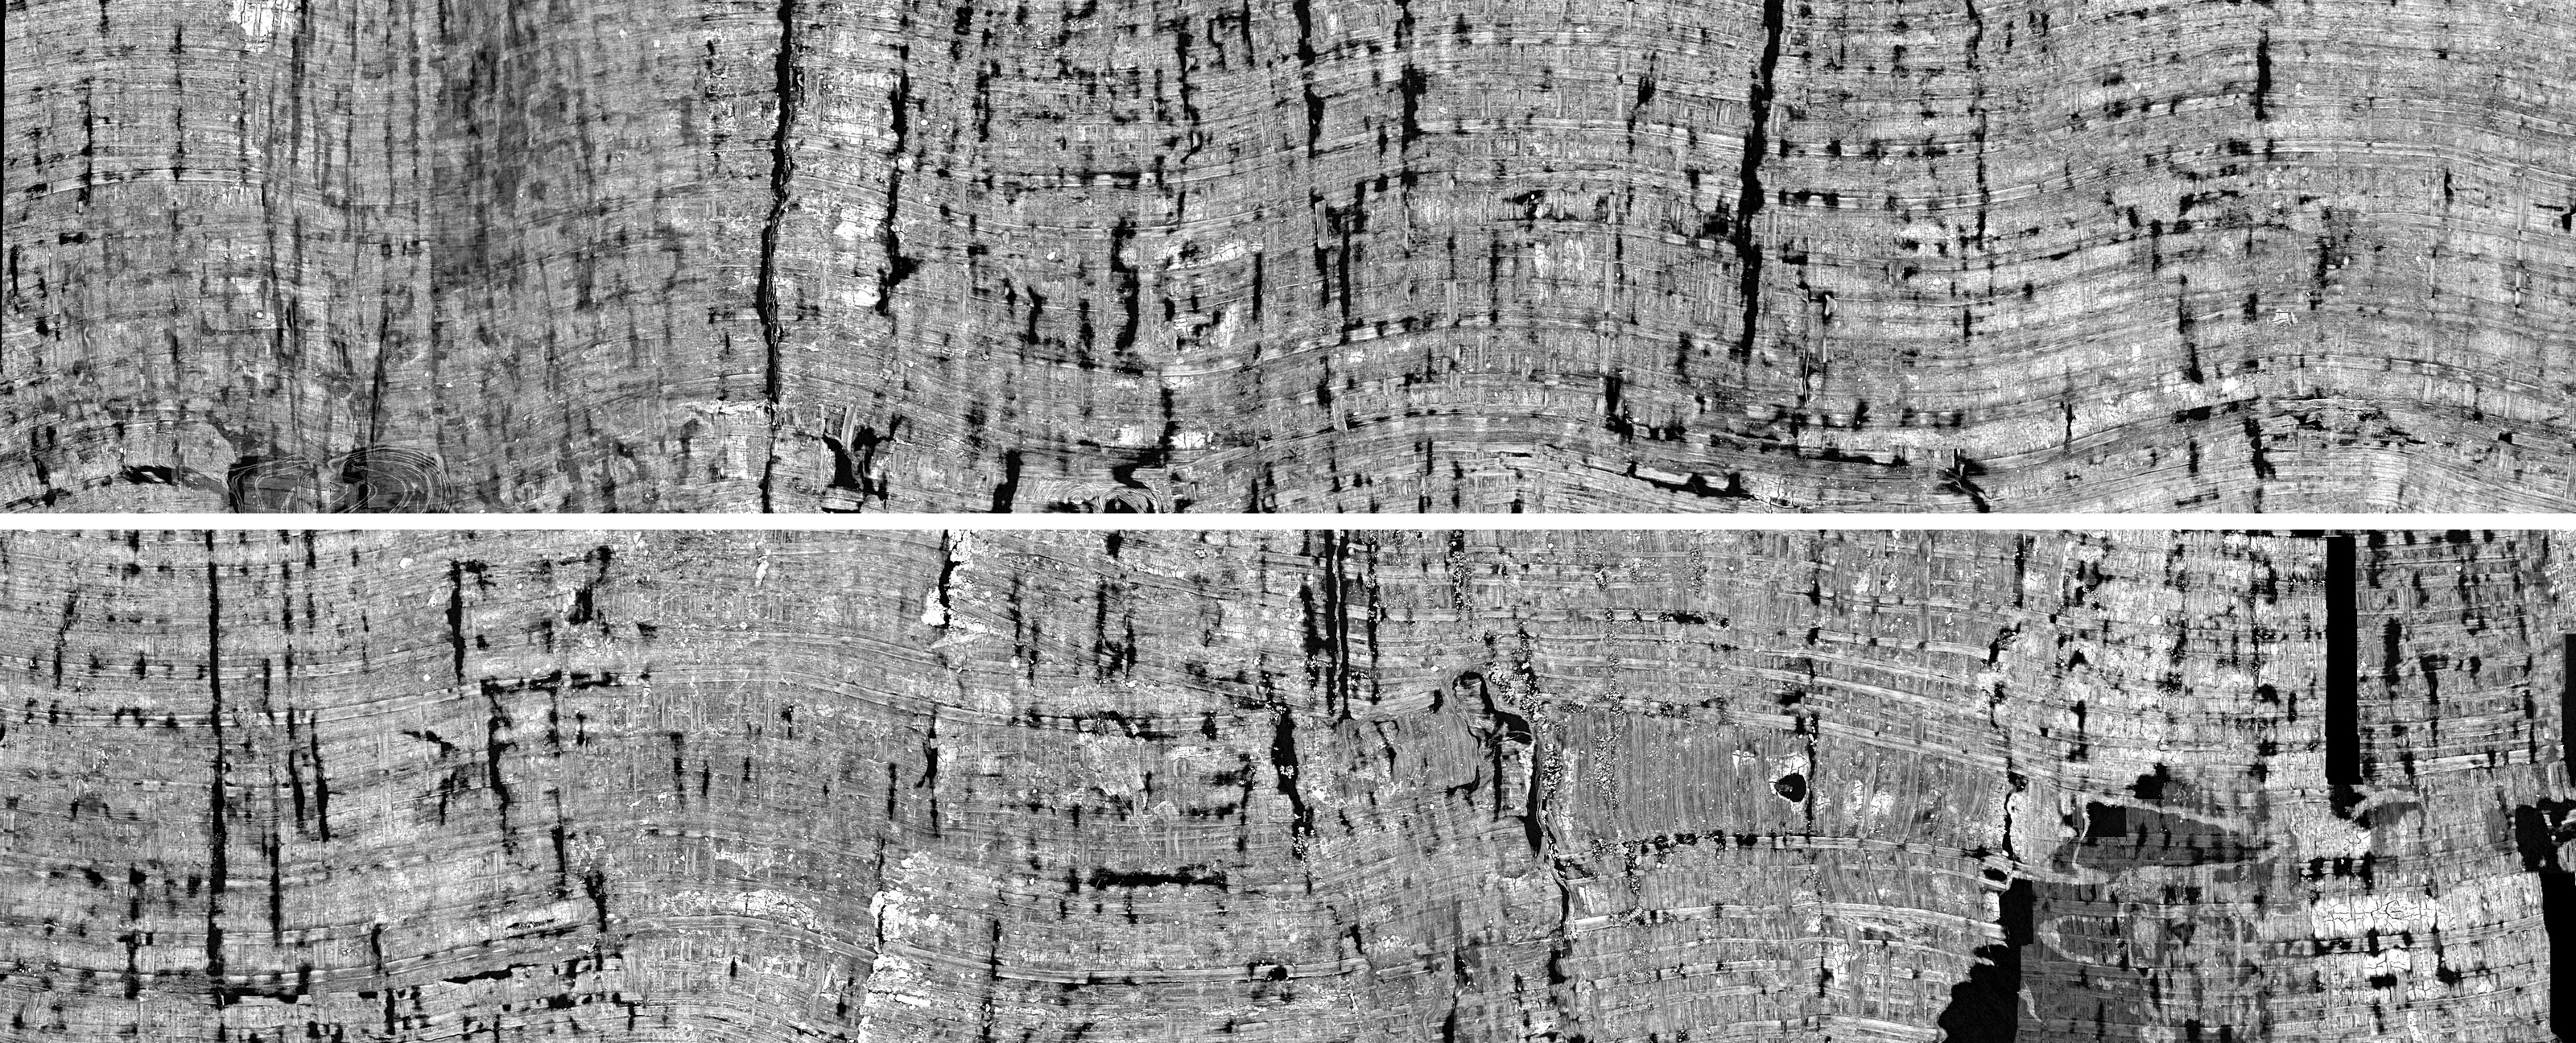
\includegraphics[width=\linewidth]{figures/quadribbon_10x10x10_hybrid_strip.jpg}
    \caption{Largest coherent readable strip: the $10^3$ hybrid champion.}
  \end{subfigure}

  \vspace{0.7em}
  \begin{subfigure}[t]{0.36\textwidth}
    \centering
    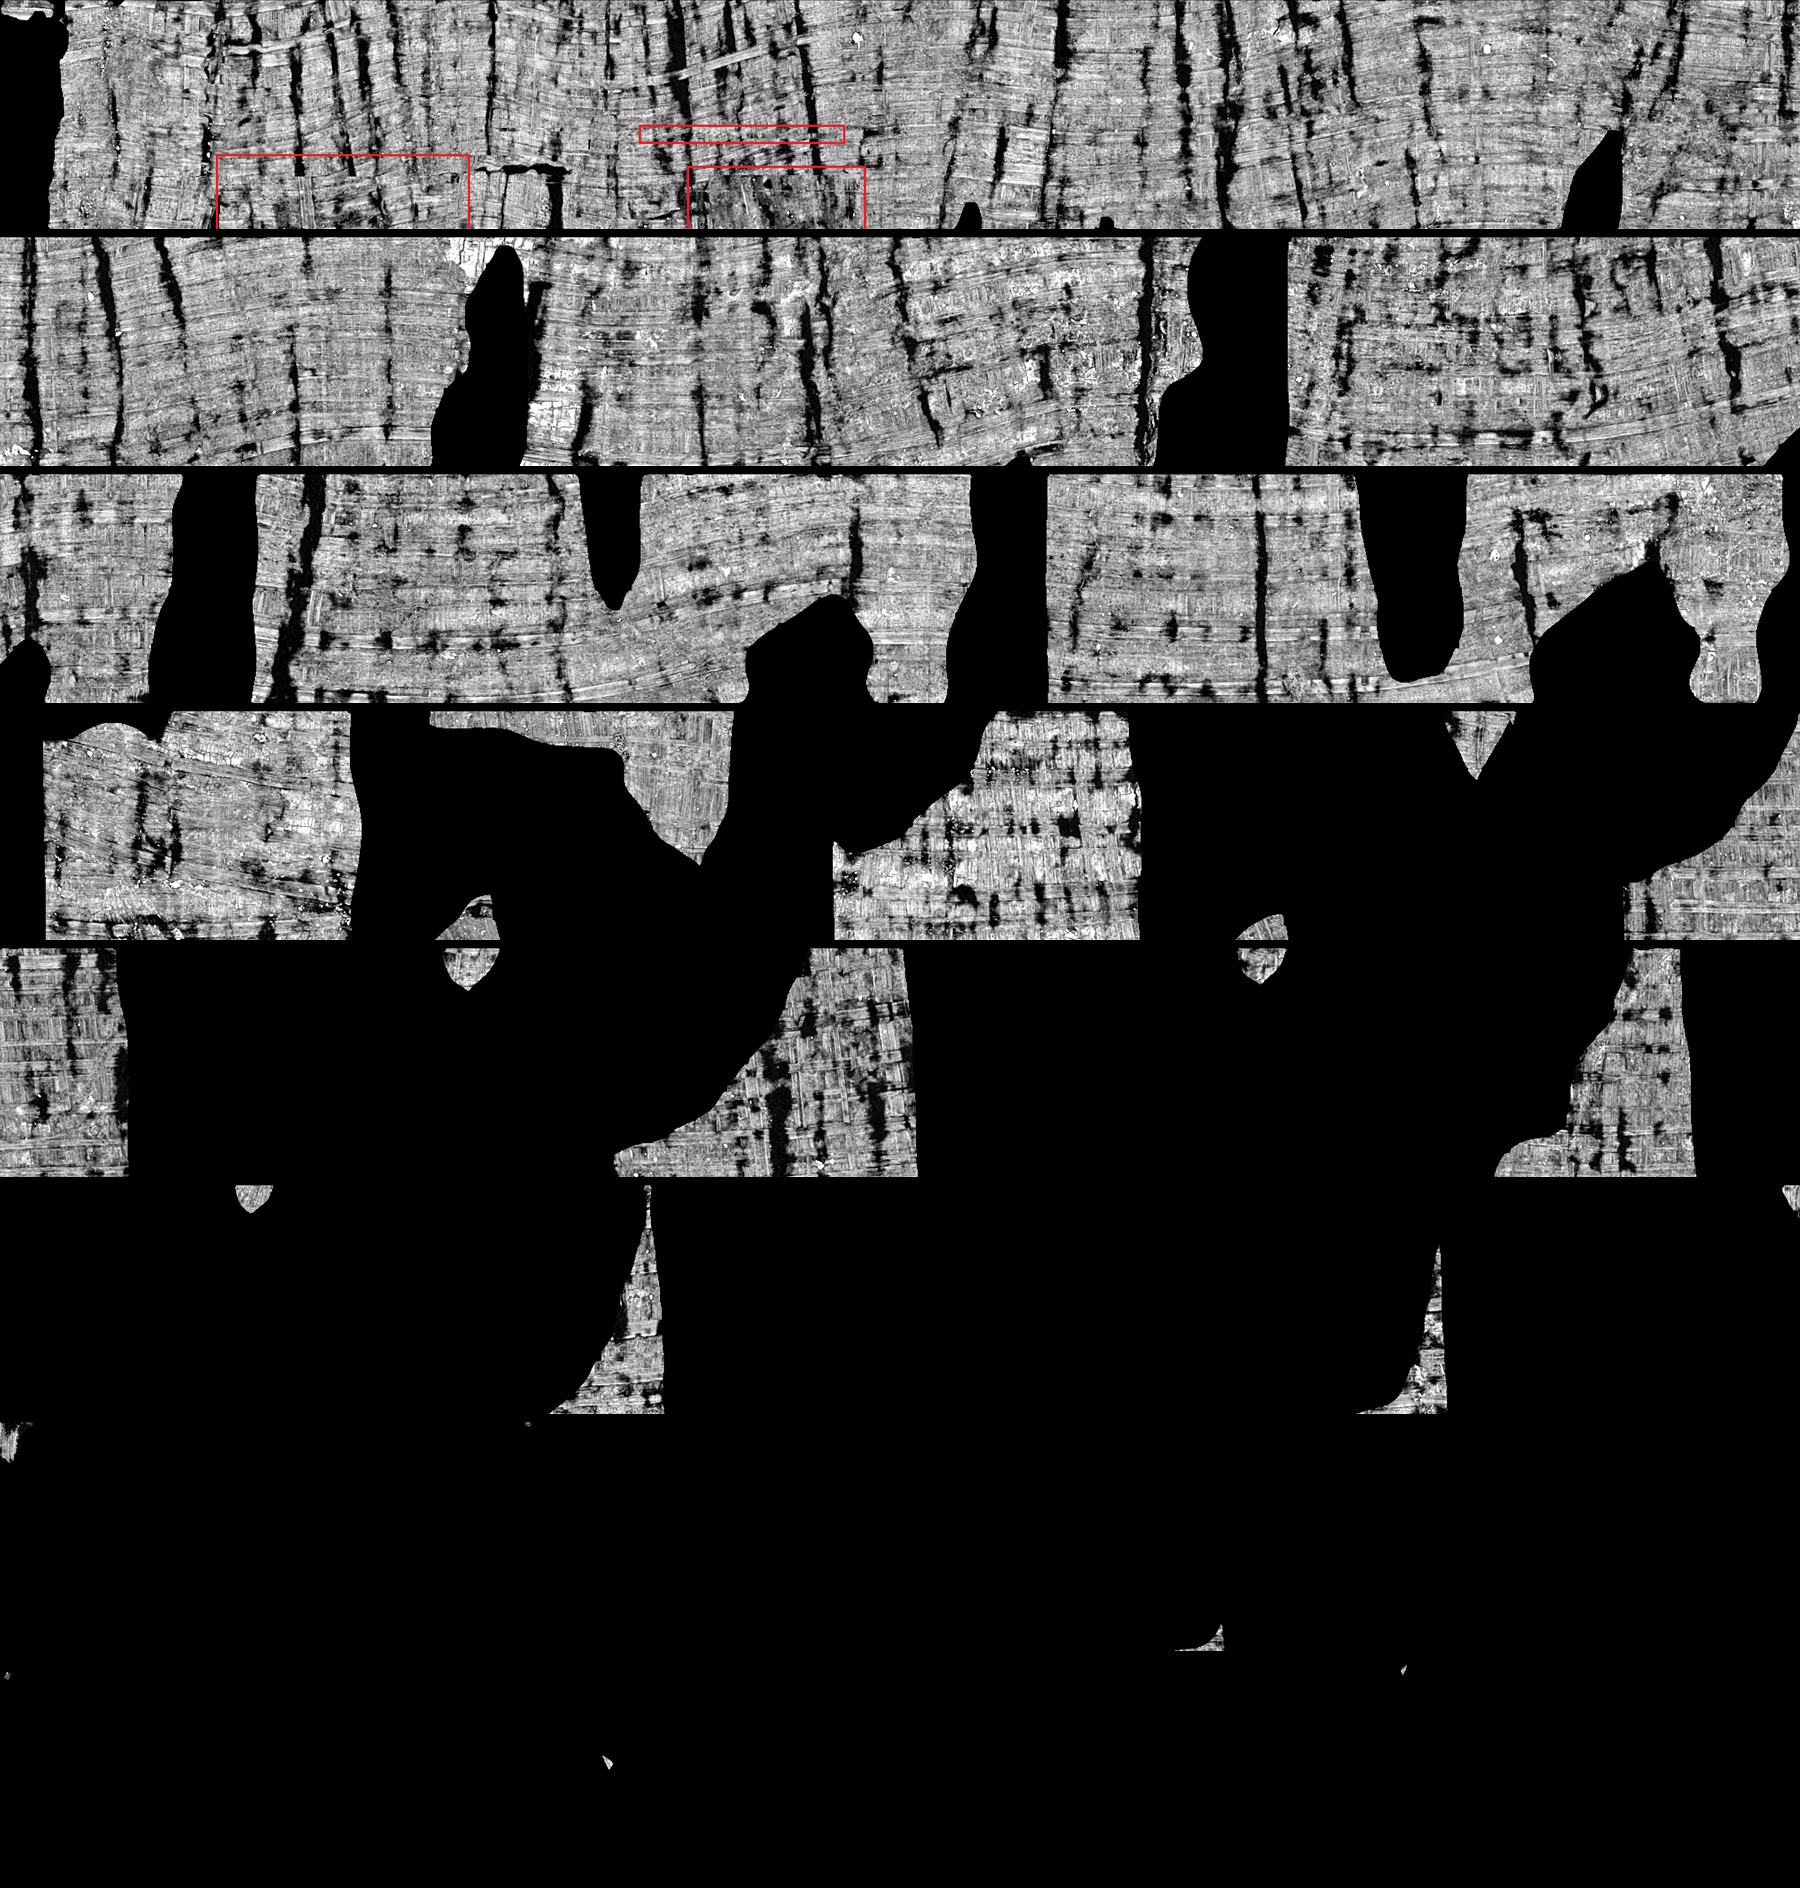
\includegraphics[width=\linewidth]{figures/quadribbon_4x5x5_page.jpg}
    \caption{Current $4\times5\times5$ integrated quadribbon page.}
  \end{subfigure}
  \hfill
  \begin{subfigure}[t]{0.55\textwidth}
    \centering
    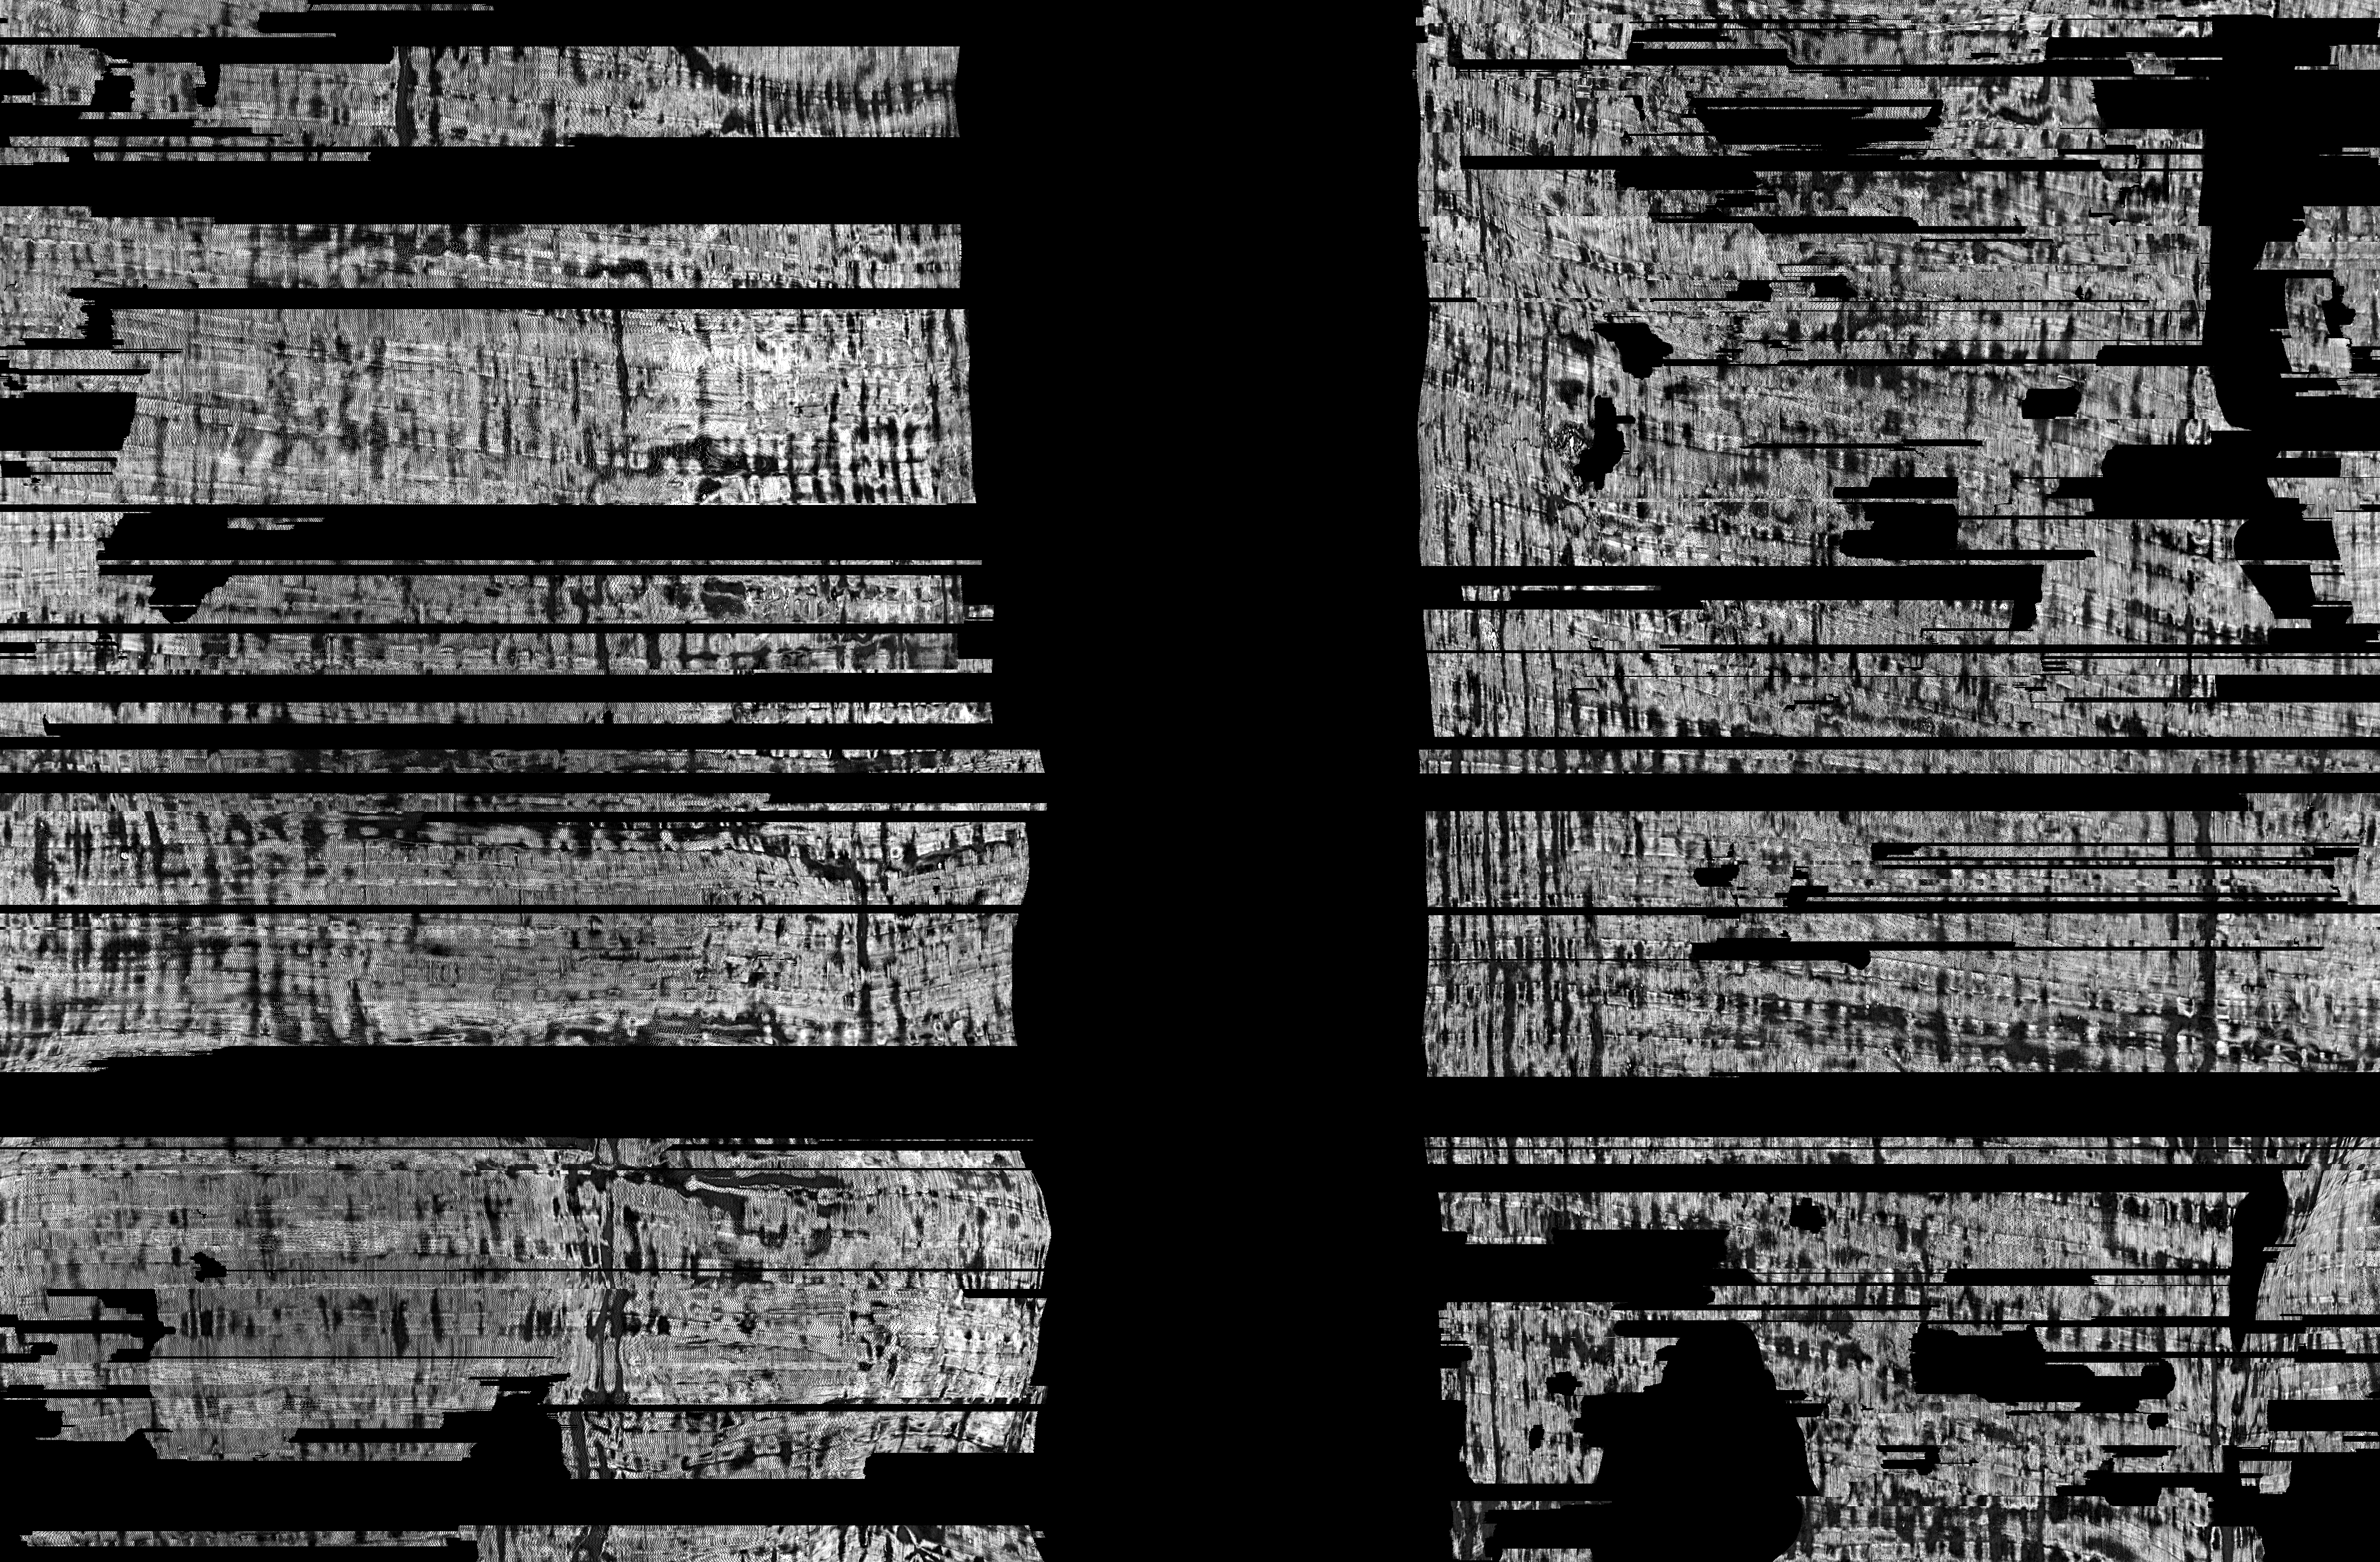
\includegraphics[width=\linewidth]{figures/sheetbook_wind50.png}
    \caption{One winding page from the full $21^3$ sheet book.}
  \end{subfigure}
  \caption{PHerc0139 scale exhibit. The top strip is the visually strongest
  coherent result, while the lower-right panel reaches the largest evidence
  extent without pretending that separated tracks are one fitted
  surface. Black regions are places with no accepted track. Separately, the current
  $21^3$ pre-fit mesh pile contains 9,110 unique world-frame contributors and
  stops before global quadribbon fit.}
  \Description{A wide coherent CT ribbon is shown above a smaller multi-row
  quadribbon page and a large winding page assembled from many
  horizontal papyrus fragments; black gaps mark absent material.}
  \label{fig:gallery-pherc0139-scale}
\end{figure*}

\begin{figure*}[p]
  \centering
  \begin{subfigure}[t]{0.485\textwidth}
    \centering
    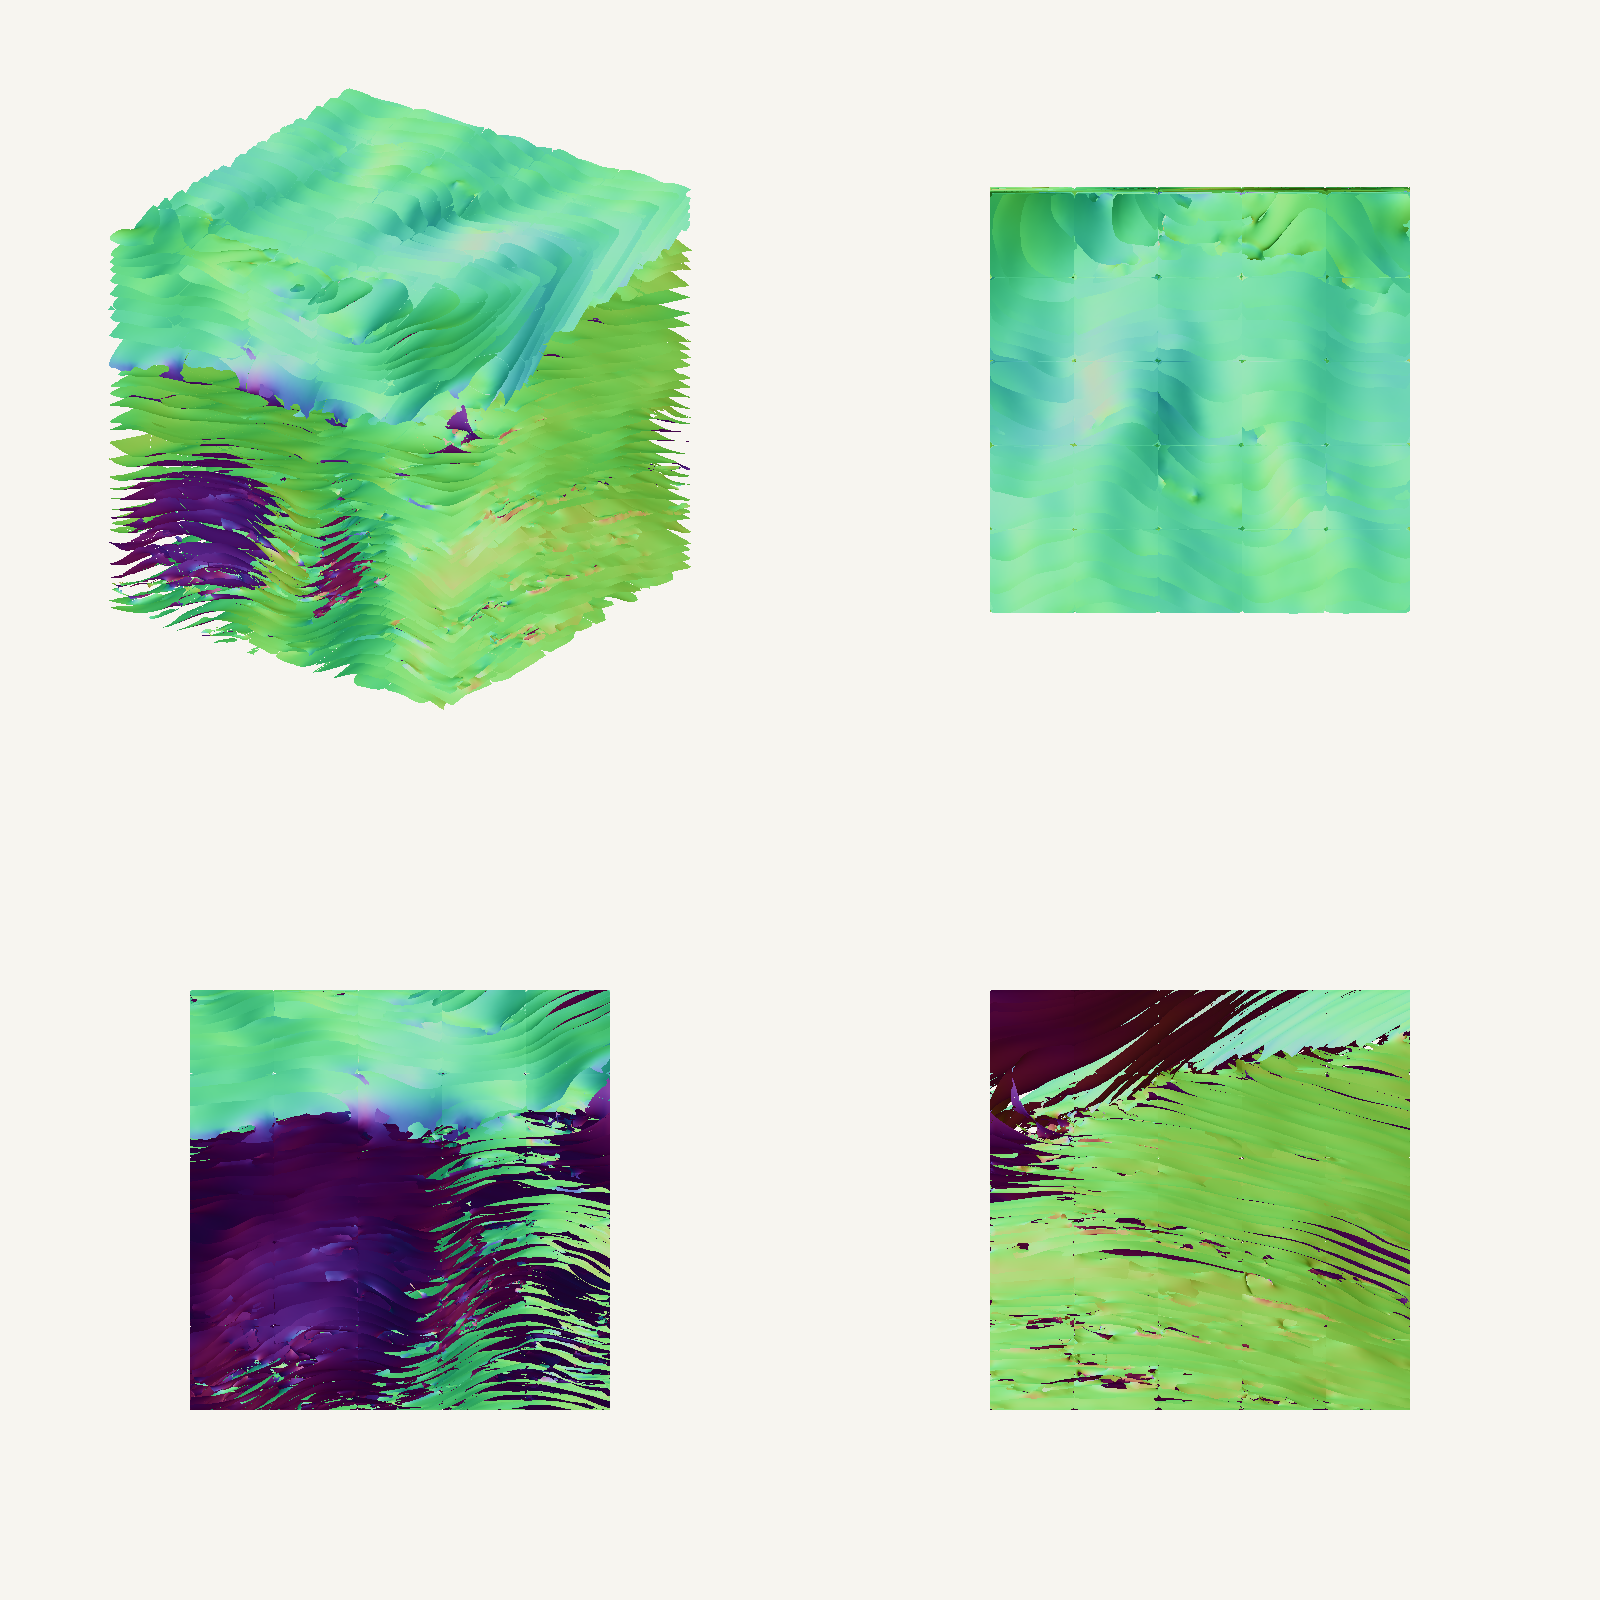
\includegraphics[width=\linewidth]{figures/prize_pherc1203_5x5x5_views.png}
    \caption{PHerc1203: 125/125 current-pipeline cube meshes.}
  \end{subfigure}
  \hfill
  \begin{subfigure}[t]{0.485\textwidth}
    \centering
    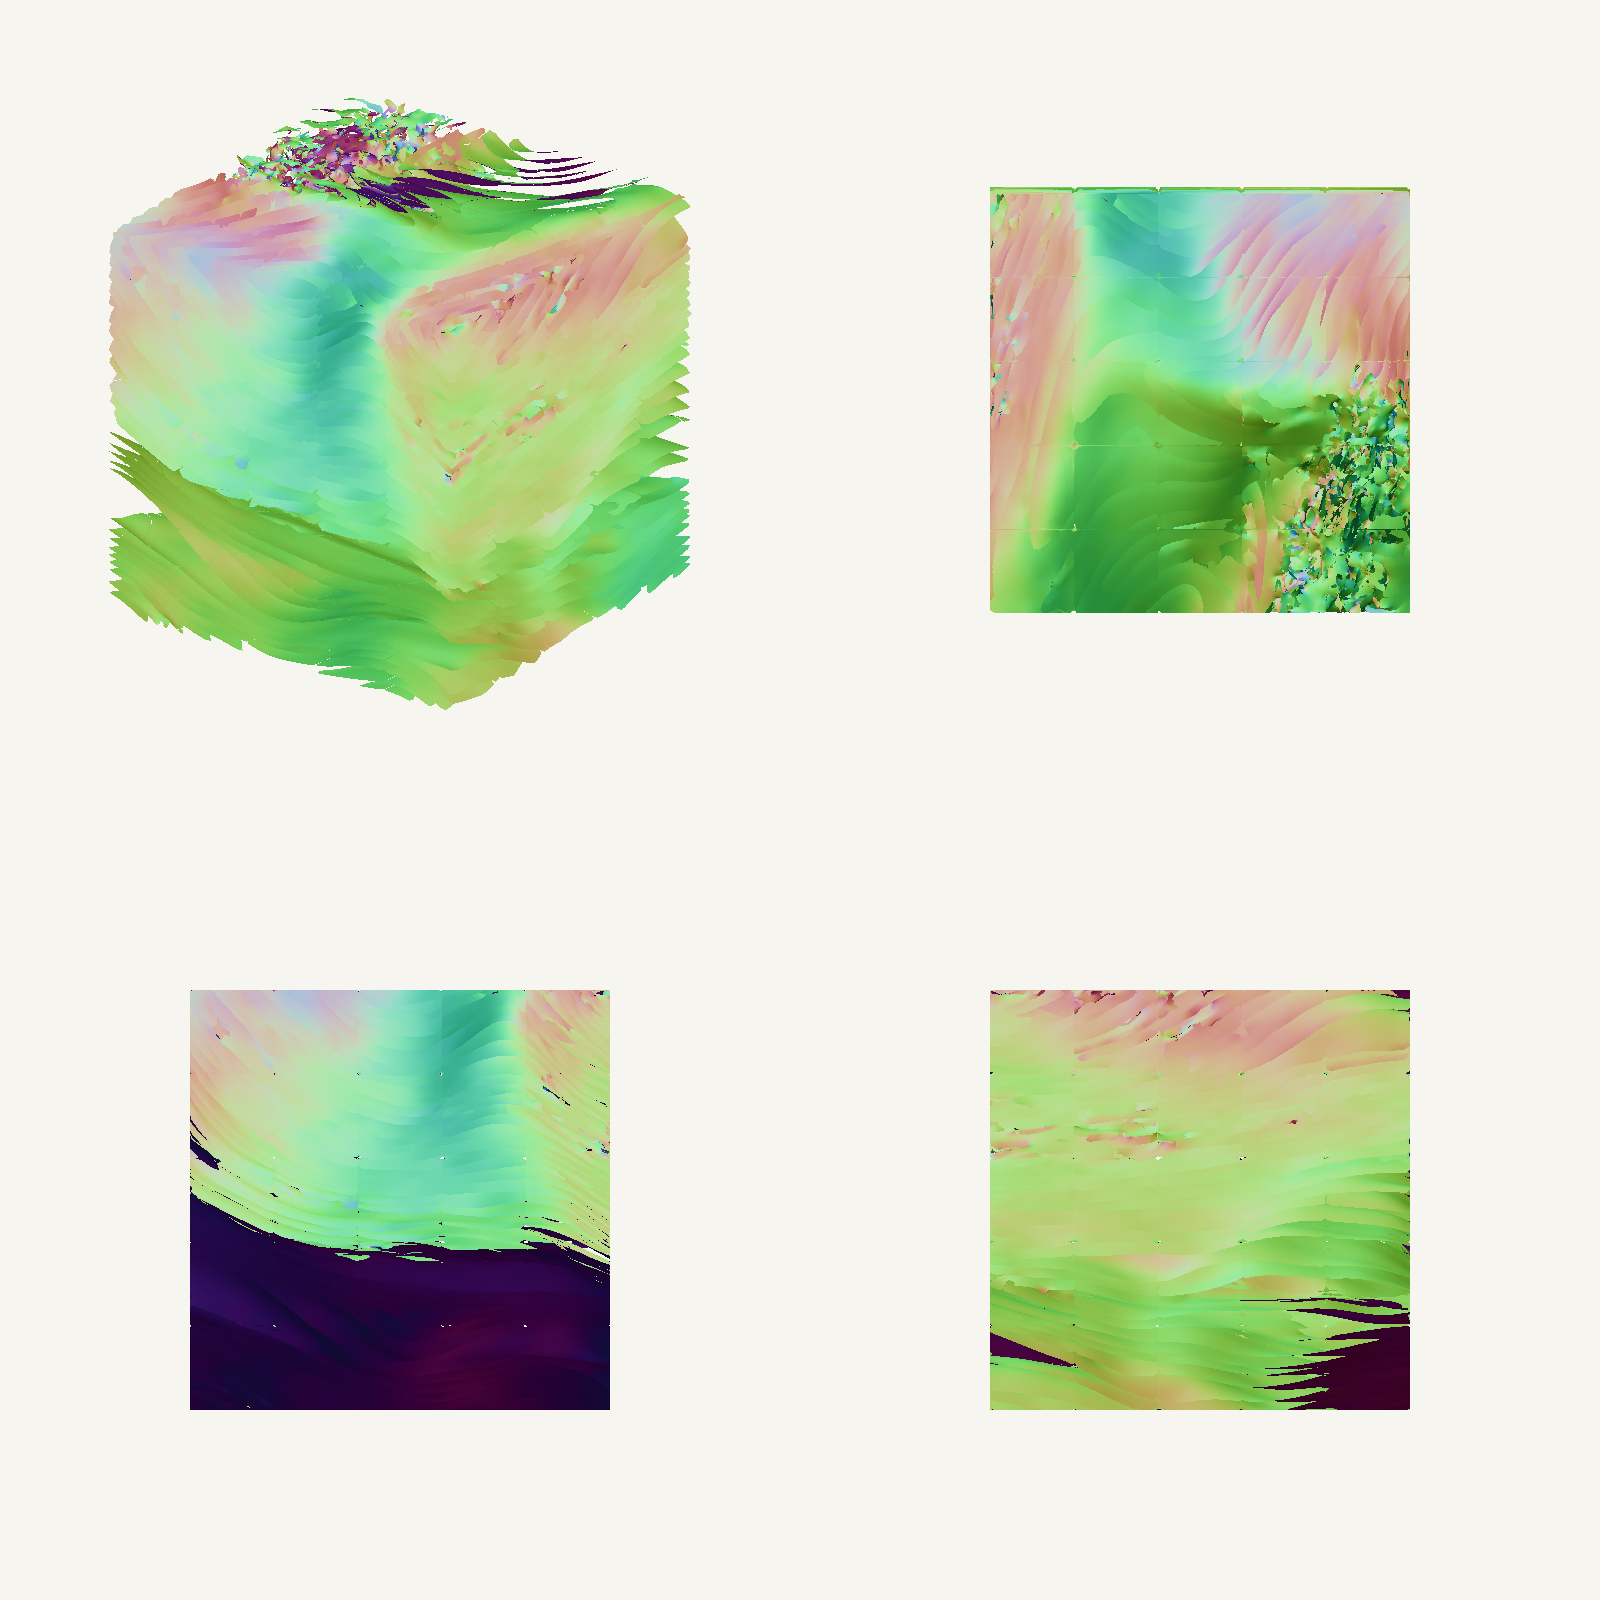
\includegraphics[width=\linewidth]{figures/prize_pherc1447_5x5x5_views.png}
    \caption{PHerc1447: 125/125 current-pipeline cube meshes.}
  \end{subfigure}

  \vspace{0.8em}
  \begin{subfigure}[t]{0.485\textwidth}
    \centering
    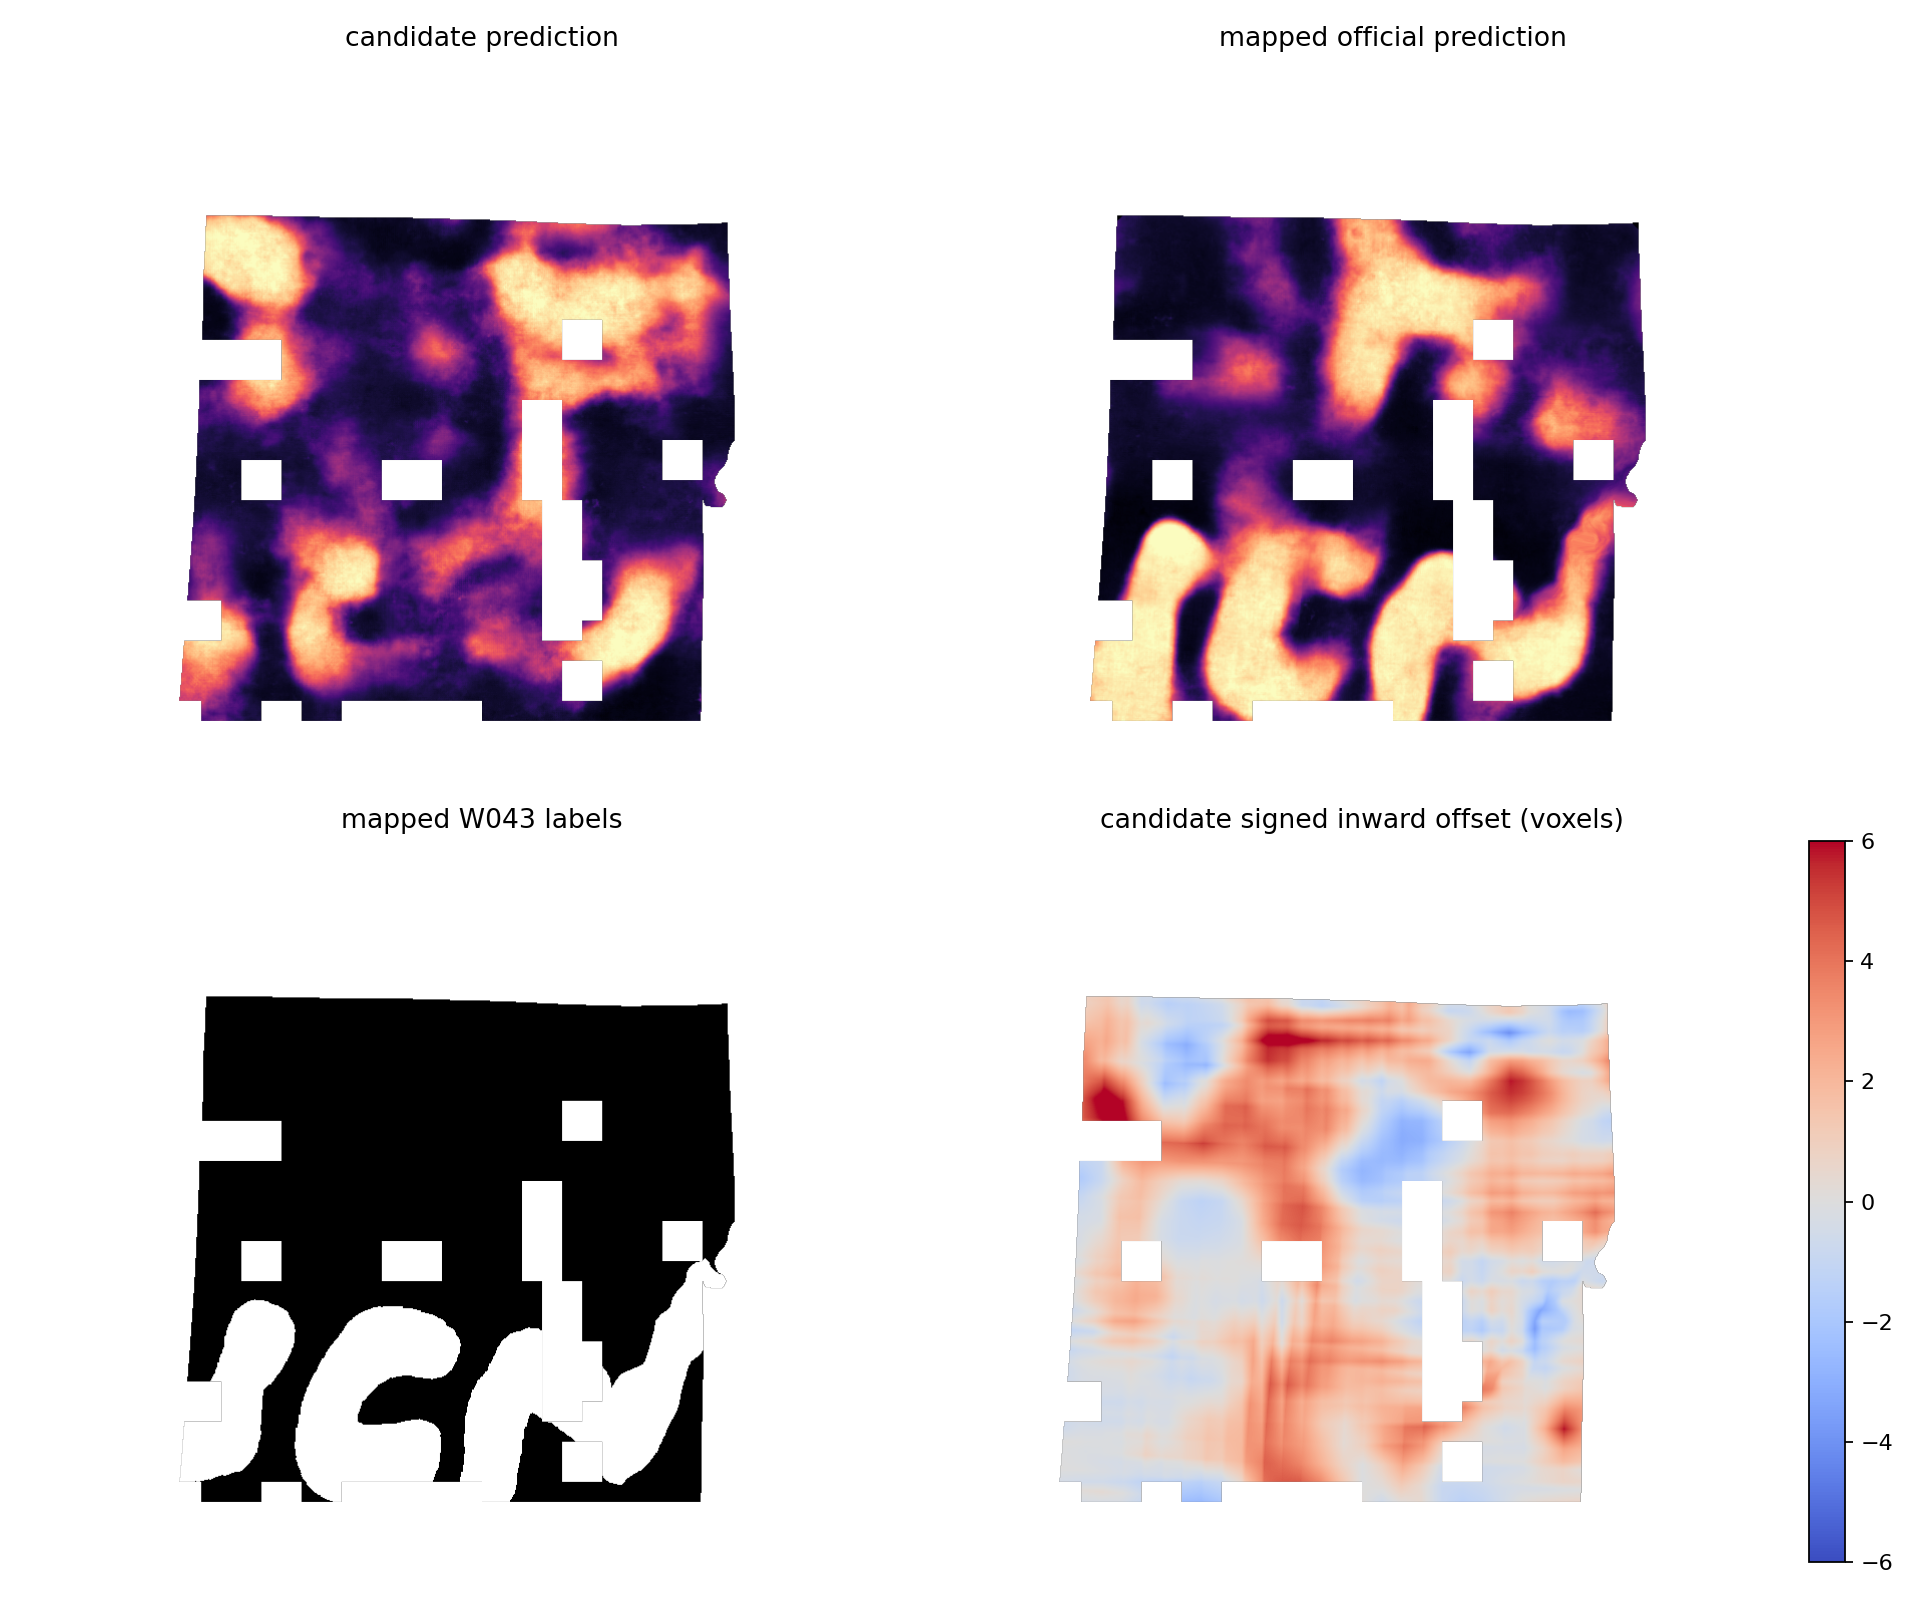
\includegraphics[width=\linewidth]{figures/w043_original_geometry_audit.png}
    \caption{W043 detector output on unchanged source geometry.}
  \end{subfigure}
  \hfill
  \begin{subfigure}[t]{0.485\textwidth}
    \centering
    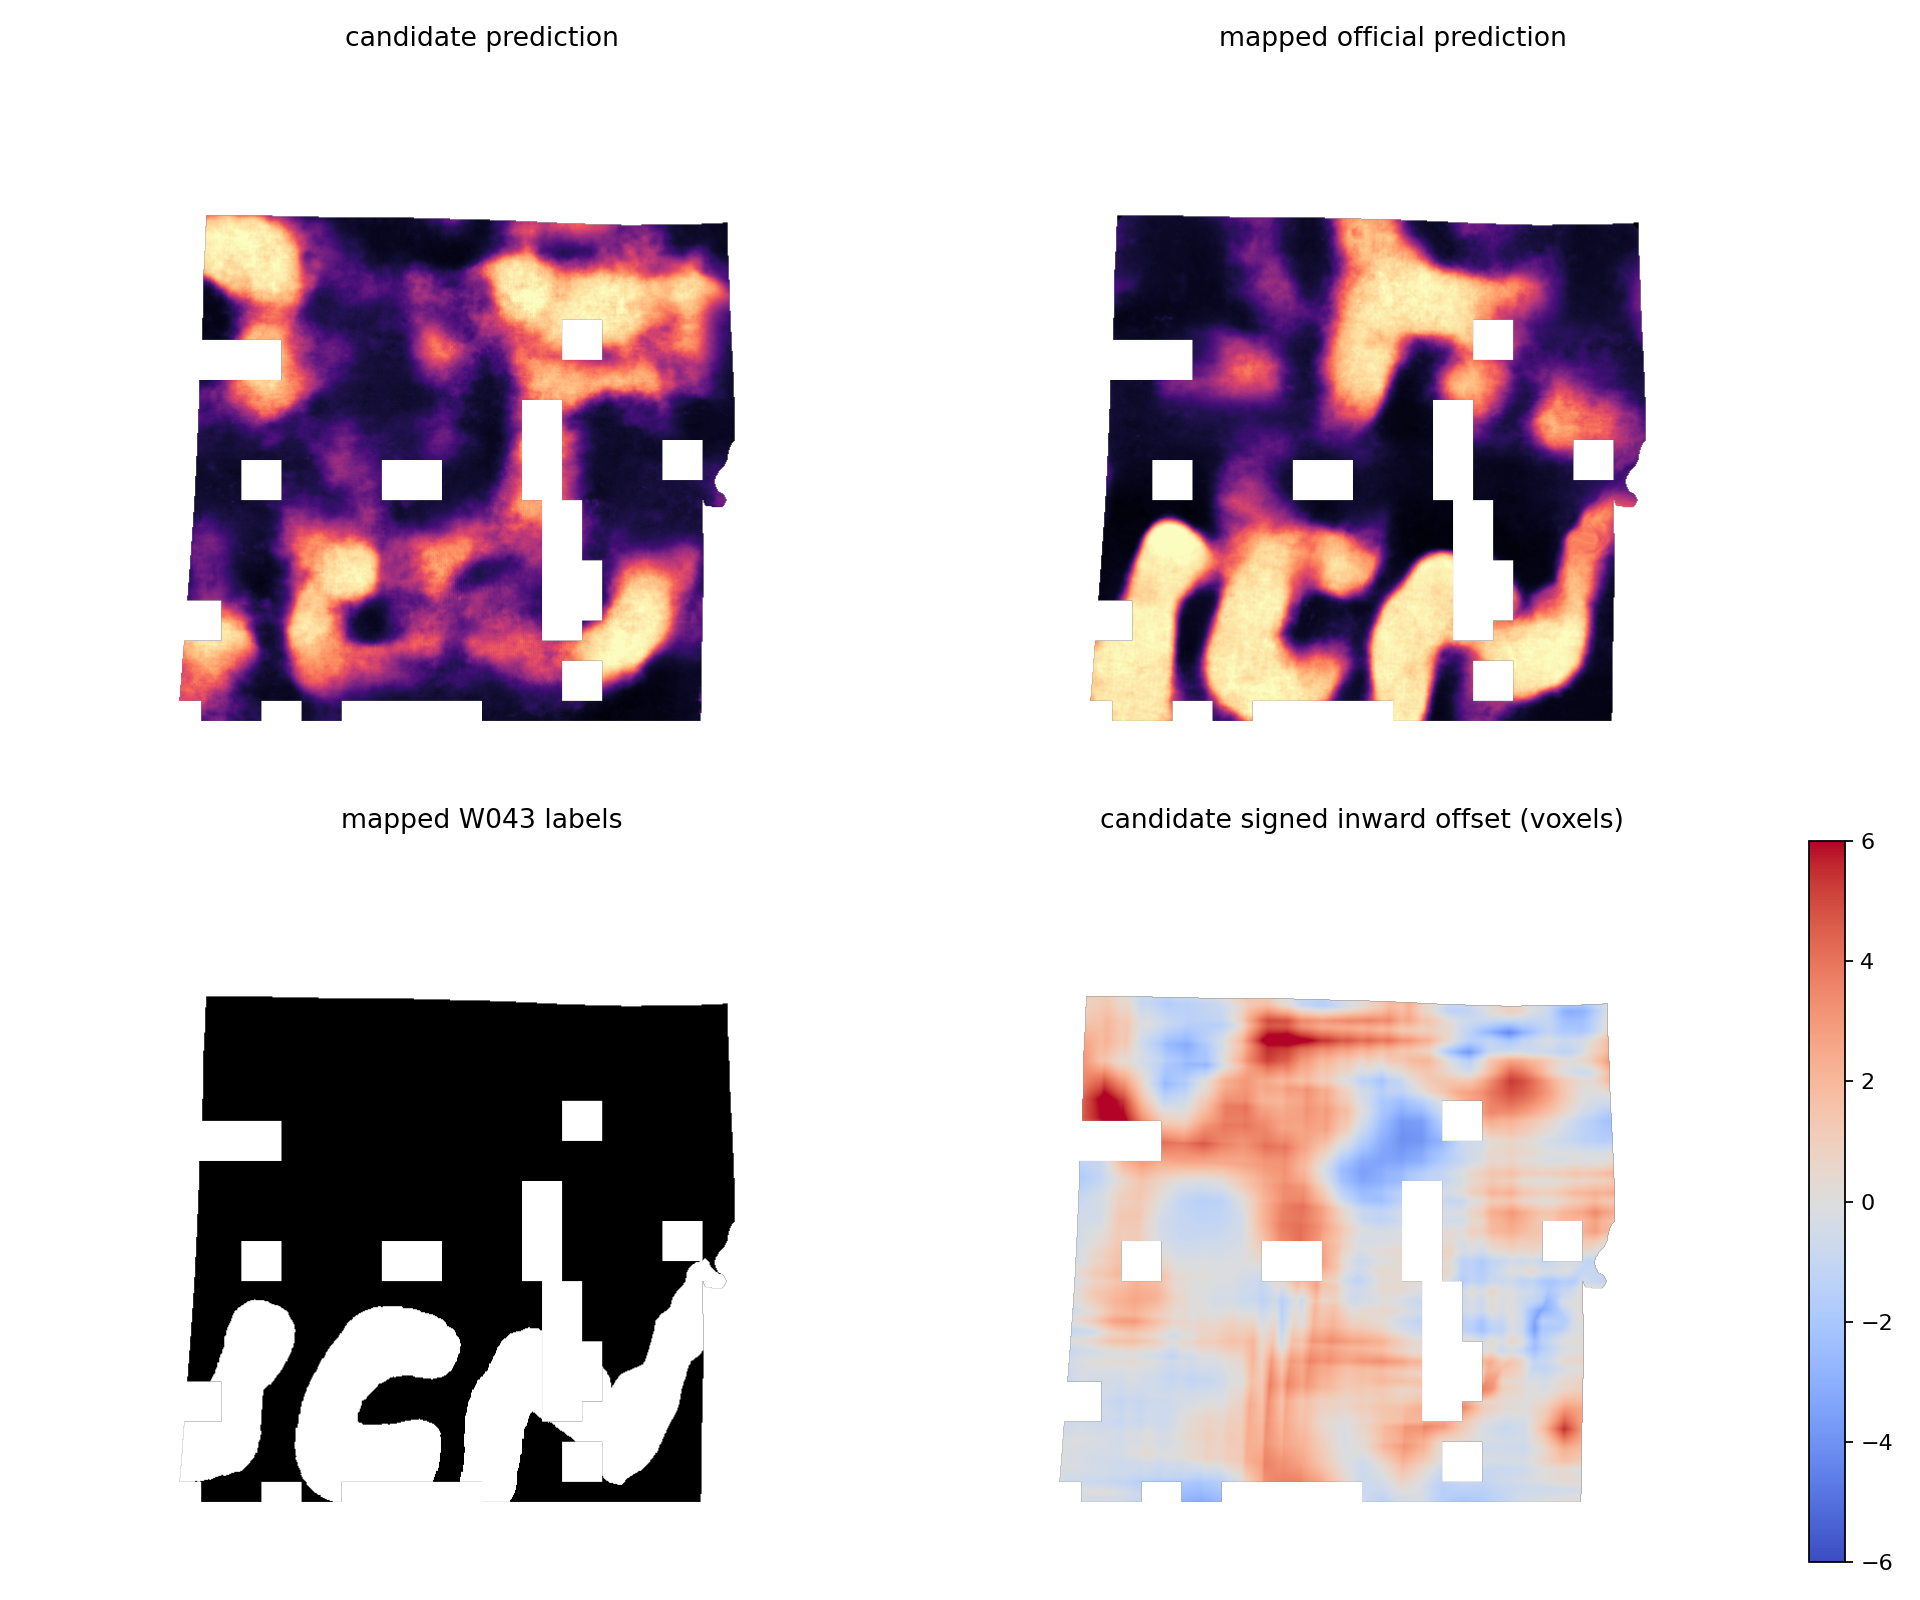
\includegraphics[width=\linewidth]{figures/w043_native_sheet_fit_audit.png}
    \caption{The same detector after native 9.362-$\mu$m normal-only fitting.}
  \end{subfigure}
  \caption{Cross-scroll transfer and downstream utility. The upper row shows
  the complete geometry-only $5^3$ prize-target piles in isometric, top, front,
  and side views; colour is view-dependent normal shading, not a confidence or
  material label. No weld or global fit has been applied. In the lower row,
  native W043 fitting improves median signed offset from $+0.810$ to $+0.395$
  voxels, normal-offset RMSE from 2.027 to 1.806, and supervised AUC from 0.6901
  to 0.7098. This is a measured, modest improvement rather than oracle
  recovery.}
  \Description{Two four-view renderings show dense stacks of curved papyrus
  surfaces for PHerc1203 and PHerc1447. Beneath them, paired W043 detector panels
  compare candidate ink probability, mapped official prediction, labels, and
  signed geometry offset before and after target-scan fitting.}
  \label{fig:gallery-transfer}
\end{figure*}
\clearpage

The public exhibit preserves the corresponding counts, topology audits,
stage boundary, and SHA-256 checksums in
\path{submission_update/gallery/}. The 6.46-GiB PHerc0139 stage-1 VMesh is
not duplicated into the paper repository; its checksum and cube-ledger totals
are published instead. The prize regions contain prediction-derived geometry
only, so no prize-scroll texture or ink claim is made.
